% mm.tex
% Author: R.R. Toledo, G.Danezis
% Revisions: 
%             March 2016 -  April 2017

\documentclass{llncs}
\usepackage{etex}
\usepackage{framed}
\usepackage{multirow}
\usepackage{tabularx}
\usepackage[ruled,algosection,noend,linesnumbered]{algorithm2e}
\usepackage{booktabs} 
\usepackage{adjustbox}
\usepackage{mathtools}
\DeclarePairedDelimiter{\ceil}{\lceil}{\rceil}
\DeclarePairedDelimiter\floor{\lfloor}{\rfloor}
\usepackage{amsfonts}
\usepackage{stmaryrd}
\usepackage{amsmath}
\usepackage{amssymb}
\let\proof\relax
\let\endproof\relax
\usepackage{amsthm}
\usepackage{color}
\usepackage{float}

\usepackage{tikz}
\usetikzlibrary{shapes, positioning, matrix, backgrounds, decorations.pathreplacing}

\newenvironment{subproof}[1][\proofname]{%
  \renewcommand{\qedsymbol}{$\blacksquare$}%
  \begin{proof}[#1]%
}{%
  \end{proof}%
}

\newtheorem{privdef}{Privacy Definition}
\newtheorem{secthm}{Security Theorem}
\newtheorem{seclem}{Security Lemma}
\newtheorem{seccjt}{Security Conjecture}

\newcommand{\todo}[1]{\textcolor{red}{TODO: #1}}
\newcommand{\raphael}[1]{\textcolor{blue}{Raphael: #1}}
\newcommand{\george}[1]{\textcolor{green}{George: #1}}

\pagenumbering{arabic}

\begin{document}
\title{Mix-ORAM: Using delegated shuffles.}

\author{   Raphael R. Toledo\inst{1}  \and George Danezis\inst{1}  \and Isao Echizen\inst{2}}
\institute{University College London, United Kingdom, \and National Institute of Informatics, Japan\\
\email{r.toledo@cs.ucl.ac.uk},\ \email{g.danezis@cs.ucl.ac.uk},\ \email{iechizen@nii.ac.jp}}

\maketitle

\begin{abstract}
Oblivious RAM is a key technology for privately querying on untrusted storage but is commonly considered impractical due to its high eviction overhead the client incurs. We propose in this work to delegate the eviction to semi-trusted third parties by presenting four different designs inspired by mix-net technologies. \todo{results}
\end{abstract}

\section{Introduction}

Cloud technologies allow impressive amounts of data to be stored on remote servers. To do so safely, not only the data integrity and confidentiality must be preserved, but also the meta data's, and so from both external adversaries and the cloud itself.
Hence, cryptographic mechanisms are used to secure communication channels, such as user authentication, data encryption and integrity checking.
These, however, do not prevent the leakage of all meta data: the servers can monitor user activities and watch which records are accessed.

Oblivious RAM (ORAM)~\cite{goldreich87}, or Oblivious Storage (OS)~\cite{boneh2011}, precisely prevents an adversary from observing the record access. In these schemes, the records are encrypted and permuted before being uploaded to the untrusted storage. When the user seeks a given record, the local client computes the corresponding remote index, fetches the encrypted data block and decrypts it. After a number of accesses, in order to render any leaked information obsolete, the database is randomized locally by the client: this is the "eviction process".

This eviction is the main bottleneck of ORAM. Indeed, the randomization consists in the whole database being permuted and its encryption refreshed so that an adversary gains no insight on the new record indices. As we assume the number of records stored remotely being orders of magnitude higher than what the client can store, the client has to download and process the database in chunks, and do so several times so that all order is equally likely. Thus as the the database size grows, the randomization cost rises super linearly.

This is why we propose to delegate the eviction process to dedicated semi-trusted parties. By chance another technology, Mix networks~\cite{chaum1981untraceable}, aims at making messages indistinguishable thanks to similar randomization done over several mixes. For the adversary to be able to link the mix-net's input and output, all of the mixes have to be compromised.
Mix-nets inspired designs can thereby be used to implement ORAM randomization process.\\

In this work, we present several privacy friendly distributed systems inspired by mix-nets to safely delegate ORAM's randomization process to semi-trusted third parties.
Their advantages include the reduction of the client computation, the possibility to delay the eviction to quieter times, the database availability during the eviction process regardless of the ORAM design and the independence from centralized parties. However careful design is required to make them scalable. Our contributions are as follows:
\begin{itemize}
 \item We introduce and motivate the use of mix-net to construct delegated ORAM schemes, that may be used by very thin clients.
 \item We present a number of designs, improve them with load balancing via parallel mixing and compare their costs and efficiency.
 \item We finally evaluate the performance of our designs with an open source implementation showing that \todo{add results here}.
\end{itemize}

We present the related work, the ORAM model, its associated threat model and explaining the different costs in Section~\ref{Related} and~\ref{Prelim}, we use random transposition shuffles them in ORAM and together with a mixnet and discuss various optimizations in Section~\ref{Mix-ORAM}. We then present our implementation, compare the costs and evaluate our designs in Section~\ref{Evaluation} before concluding.

\section{Related Work}\label{Related}
\noindent\textbf{ORAM.}
ORAM was first presented by Goldreich and Ostrovsky in 1990~\cite{ostrovsky1990efficient} to prevent reverse engineering and protect software running on tamper resistant CPUs. The model was formally extended in 2011~\cite{boneh2011} to data protection on untrusted remote clouds.
Since then, enhancement have been proposed including \textit{data structures} diversification~\cite{goldreich1996software,stefanov2011towards,stefanov2013path,ren2014ring},
the use of more and more sophisticated \textit{security definitions} with statistical security~\cite{damgaard2011perfectly,ajtai2010oblivious} and differential privacy~\cite{wagh2016root}, and the revision of \textit{item lookups} with cuckoo hashing~\cite{pinkas2010oblivious} and bloom filters~\cite{williams2008building}.
Most ORAM constructions are based on a single client-server model, but multi-user designs were gradually introduced \cite{backesanonymous,franz2011oblivious,goodrich2012privacy}.\\

\noindent\textbf{Shuffling and Sorting.}
Shuffle and sorting algorithms are a thoroughly researched subject central to ORAM for the randomization process. However most of the existing methods are not useful for ORAM as they are not oblivious in that the permutations done depends on the data itself.
Examples of oblivious sorting algorithms include sorting networks such as Batcher's~\cite{batcher1968sorting} and the ones based on AKS~\cite{ajtai19830}, which unfortunately were proven to be impractical because of the high number of I/Os, but also more recent and efficient ones~\cite{paterson1990improved}.
Newer designs include the randomized Shellsort~\cite{goodrich2010randomized}, an elegant simple data-oblivious version of the Shellsort algorithm, the Zig Zag sort~\cite{goodrich2014zig} presented in 2014, the Melbourne shuffle~\cite{ohrimenko2014melbourne} and work of particular interest written by Goodrich in 2012~\cite{goodrich2012anonymous} assess the information leakage due the use of a partially compromised parallel mix-net.\\

\noindent\textbf{Mix-nets.}
Mix-nets were first presented for anonymous e-mailing by David Chaum in 1981~\cite{chaum1981untraceable}. As they became popular many improvements were made over the years~\cite{moller2003mixmaster,danezis2003mixminion,danezis2004minx,danezis2009sphinx}. Mix-nets' main goal is to give users anonymity by hiding the correspondence between the incoming users' packets and the mix-nets output. To do so, the users' messages go through several mixes which permute them and refresh their encryption. Either reencryption~\cite{wikstrom2006adaptively} and onion encryption can be used, proofs of shuffle~\cite{groth2007verifiable,groth2007non,bayer2012efficient} and Randomized Partial Checking~\cite{jakobsson2002making} can help verify the shuffle correctness.

This work is inspired by the mix-net technology for its encryption and permutation functionalities, however, only the packet unlinkability property is of interest for ORAM. From now on, we refer traditional ORAM solutions as ORAM and our designs as Mix-ORAM.

\section{Preliminaries}\label{Prelim}
%
\subsection{System}\label{System}

The Oblivious RAM system is a distributed system composed of two parties, the ORAM \emph{server} and the \emph{client} to which we add the \emph{mix-net}. The \emph{server} handles two data arrays, one we call \emph{database} and comprises the user's encrypted records, and a temporary one we call \emph{cache} of lesser size used to hide the number of times a record was accessed and only read and write operations are available.
The \emph{client} comprises a small memory in which the cache and some additional records can fit and relies on two main methods that we describe as follows. The \emph{mix-net} is responsible for handling the eviction initiated by the client.\\

\noindent\textbf{The access method:} To do a read or write operation, the client first check locally in the cache whether the desired record is present, if so a dummy record is fetched from the database else the desired record. Finally, the fetched element is encrypted if the operation is a read else overwritten with the provided data for a write operation. The element is then stored locally in the cache before it is sent back to the remote server.\\

\noindent\textbf{The eviction method:} When the cache is full, the client starts the eviction process to prevent too important information leakage. The eviction consists of two parts where the client first \textit{rebuilds} the database before starting the \textit{oblivious shuffle}, the subject of this paper.

During the \emph{rebuild phase}, the client obliviously uploads back the records from the cache back to the ORAM database. After doing so, the client can finally starts \emph{the oblivious shuffle}. The client first selects a set of mixes which will randomize the database. It then generates and sends to them randomization instructions. The mixes use these to compute the encryption keys and permutation seeds, fetch their allocated records from the database, and keep randomize them (encrypt and shuffle with the keys and seeds, forward them and start again) for a specified number of rounds before uploading them back to the database.

\subsection{Security definitions and Threat model}\label{Threat}

We presume here the existence of a motivated adversary trying to subvert a target user's privacy by learning the correspondence between the remote and the real record indices. We furthermore assume that the user protects its data with an ORAM system compliant with the Privacy Definition~\ref{def:Oram} introduced by Stefanov et al.~\cite{stefanov2011towards} and additionally that all communications between the client, ORAM server and mixes are secured but may be intercepted as in the \textit{global passive adversary} assumption.
Finally, we suppose the adversary has corrupted a number of machines to achieve their goal, unless said otherwise the ORAM server and all but one mix are considered compromised, and that the compromised machines behave in a \textit{honest but curious} way in that all operation are correctly performed but passively recorded and all secrets shared with the adversary.

\begin{privdef}\label{def:Oram}
Let $\text{seq}_k=\{(\text{op}_1, \text{ad}_1, \text{data}_1), \text{ ... },(\text{op}_k, \text{ad}_k, \text{data}_k)\}$ denote a sequence of $k$ queries, where $op$ denotes a read or write operation, $ad$ the address where to process the operation and $data$ the block to write if needs be else $\perp$.
We denote by $ORAM(seq_k)$ the resulting randomized data access from the ORAM process with input $seq_k$.
The ORAM guarantees that $ORAM(seq_k)$ and $ORAM(seq'_{k'})$ are computationally indistinguishable if $k=k'$.
\end{privdef}

This work focuses on the ORAM eviction process and more precisely on the oblivious shuffle phase where sequences of data-blocks are shuffled and encrypted in order to hide the records indices after access information has leaked. This problem refers to the eviction of the shelter in the database in the Square Root solution~\cite{ostrovsky1990efficient} and to the eviction of upper partitions in a lower ones in the Hierarchical case~\cite{goldreich1996software}. We evaluate the security of our designs by looking at the oblivious shuffle information leakage and at the correctness of the cryptography. We note by $\sigma$ the permutation seeds and $k$ the encryption keys.\\

\noindent\textbf{Model.} We consider here an ORAM remote server consisting of a database with memory of $n\ b$-bit long data blocks and a cache with memory of $s,\ s\ll n,\ b$-bit long data blocks. We furthermore consider a mix-net composed of $m$ mixes with memory of $n/m$ data blocks, and a client with memory of $s$ data blocks. The ORAM server, the mixes and the client additionally have a small memory of capacity $\mathcal{O}(m)$ to store extra information about the  permutation and encryption. We consider facing the threat of a polynomial time adversary and call $\kappa$ our security parameter representing the length of our encryption keys and seeds.\\

\noindent\textbf{Costs.} We are interested on one side in the costs incurred by the client for recovering a record index, for decrypting a record and the extra space needed, on the other side in the total costs incurred by the mixes encrypting the records, permuting them and the transferring them.
Some operations can be preprocessed by the mixes while the records are being transferred, as the key and seeds generation and the record allocation, and as thus will not be the main focus.
%
\subsection{Cryptographic Primitives}

\noindent\textbf{PRG \& Seeds.}
ORAM systems use pseudo random generators (PRG) and seeds to link remote and real indices. A distribution $\mathcal{D}$ over strings of length $l$ is said pseudo random if $\mathcal{D}$ is indistinguishable from the uniform distribution over strings of length $l$~\cite{katz2014introduction}. That means it is infeasible for any polynomial-time adversary to tell whether the string was sampled accordingly to $D$ or was chosen uniformly at random. A PRG is a deterministic algorithm that receives as an input a short random key and stretches it into a long pseudo random stream.\\\

\noindent\textbf{Encryption.}
ORAM designs heavily rely on encryption to obfuscate the records during the eviction and the  access.
The Advanced Encryption Standard (AES)~\cite{daemen2013design} has high speed and low RAM requirements: it has throughput over 700 MB/s per thread on recent CPUs such as the Intel Core i3~\cite{mcwilliams2014hardware} which makes it the ideal choice for ORAM.
We also make use of elements of a elliptic curve group of prime order satisfying the decisional Diffie-Hellman assumption to compress the instructions sent to the mixes.

\section{Mix-ORAM}\label{Mix-ORAM}
This work aims at obviously sorting the database from an old state $\Pi_{\sigma_1}(DB)$ to a new one $\Pi_{\sigma_2}(DB)$. As the seed space is not structured, the overall mix-net is limited to perform a permutation $\Pi_{\sigma'}$ such that $\Pi_{\sigma_2}(DB) = \Pi_{\sigma'} \circ \Pi_{\sigma_1} (DB)$. We present two ways to solve the problem, one called the \emph{Layered method} where there is no relation between seeds and the second the \emph{Rebuild method} where $\Pi_{\sigma'} = \Pi_{\sigma''} \circ \Pi_{\sigma_1}^{-1}$. 

In this section, we first introduce the two methods to randomize the records during the eviction over a simple cascade mix-net. We then optimize the Mix-ORAM schemes by considering a stratified mix-net together with distributed shuffle algorithms.

\subsection{A simple Mix-ORAM}\label{ASMO}
We introduce here the two randomization methods over a semi-trusted cascade mix-net. For each method, we show how the mix-net encrypts and permutes the records and how the client recovers a record plain text.

\begin{figure}[H]
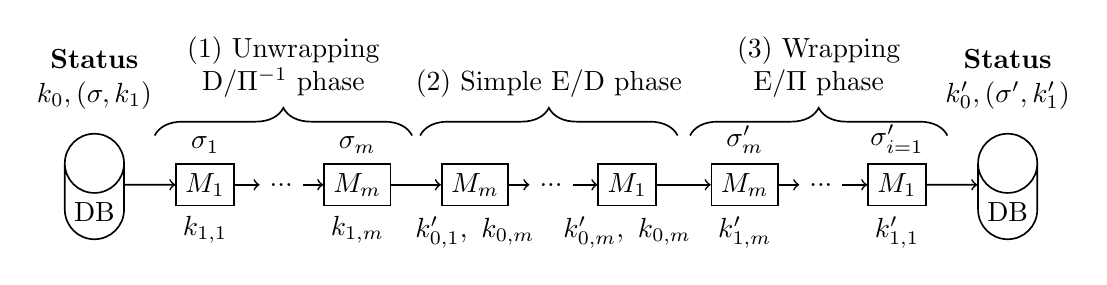
\begin{tikzpicture}[auto, semithick, node distance= 4em]
\tikzstyle{every state}=[fill=white,draw=black,thick,text=black]
\node[draw, cylinder, shape border rotate=90, minimum height=3em,minimum width=2em,  label={[align=center, yshift=0.5em]\textbf{Status} \\$k_0, (\sigma, k_1)$}]    	(X)				  {DB};
\node[draw, rectangle, align=center, label=below:{\color{white}'\color{black}$k_{1,1}$\color{white}'}, label=above:{${\sigma_{1}}$}]   		(A)[right of=X, yshift=1em]   {$M_1$};
\node[draw=none, fill=none] (XX)[right of=A, xshift=-1.25em] {...};
\node[draw, rectangle, align=center, label=below:{\color{white}'\color{black}$k_{1,m}$\color{white}'}, label=above:{${\sigma_{m}}$}]   		(AA)[right of=XX, xshift=-1.25em]   {$M_m$};
\node[draw, rectangle, align=center, label=below:{$k_{0,1}',\ k_{0,m}$}]    		(B)[right of=AA, xshift=.25em]    { $M_m$};
\node[draw=none, fill=none] (XXX)[right of=B, xshift=-1.25em] {...};
\node[draw, rectangle, align=center, label=below:{$k_{0,m}',\  k_{0,m} $}]    		(BB)[right of=XXX, xshift=-1.25em]   { $M_1 $};
\node[draw, rectangle, align=center, label=below:{$k_{1,m}'$}, label=above:{$\sigma_{m}'$}]    		(C)[right of=BB, xshift=.25em]   {$M_m$};
\node[draw=none, fill=none] (YY)[right of=C, xshift=-1.25em] {...};
\node[draw, rectangle, align=center, label=below:{$k_{1,1}'$}, label=above:{$\sigma_{i=1}'$}]    		(CC)[right of=YY, xshift=-1.25em]   {$M_1$};
\node[draw, cylinder, shape border rotate=90, minimum height=3em,minimum width=2em, label={[align=center, yshift=0.5em] \textbf{Status}\\$k_0', (\sigma', k_1')$}]    	(Y)[right of=CC,yshift=-1em]	  {DB};

\draw[decoration={brace, amplitude=1em}, decorate]  ([yshift=1em, xshift=-.75em]A.north west) -- ([yshift=1em,xshift=.75em]AA.north east) node[above, pos=0.5, yshift=1em, align=center] {(1) Unwrapping \\ D/$\Pi^{-1}$ phase};
\draw[decoration={brace, amplitude=1em}, decorate]  ([yshift=1em, xshift=-.75em]B.north west) -- ([yshift=1em,xshift=.75em]BB.north east) node[above, pos=0.5, yshift=1em] {(2) Simple E/D phase};
\draw[decoration={brace, amplitude=1em}, decorate]  ([yshift=1em, xshift=-.75em]C.north west) -- ([yshift=1em,xshift=.75em]CC.north east) node[above, pos=0.5, yshift=1em, align=center] {(3) Wrapping \\ E/$\Pi$ phase};

\path[->]
([yshift=1em]X.east) edge     	node{}    	(A.west)
(A.east) edge     	node{}    	(XX.west)
(XX.east) edge		node{}		(AA.west)
(AA.east) edge		node{}		(B.west)
(B.east) edge		node{}		(XXX.west)
(XXX.east) edge		node{}		(BB.west)
(BB.east) edge     	node{}    	(C.west)
(C.east) edge     	node{}    	(YY.west)
(YY.east) edge     	node{}    	(CC.west)
(CC.east) edge     	node{}    	([yshift=1em]Y.west);
\end{tikzpicture}
\centering
\caption{Eviction method with the encryptions $k$ and permutations seeds $\sigma$. } \label{fig:eviction}
\end{figure} 


\subsubsection{Layered Cascade scheme.}
In this scheme, we use the the layered encryption method over the cascade mix-net for the eviction of the database. The underlying principle of the layered method is to have the whole database go through mix-net once, each mix adding layers of encryption and permutation on top of the records which corresponds to the sole Wrapping phase (1) of Figure~\ref{fig:eviction}.

Before uploading for the first time the data to the ORAM server, the client prepares the records by appending to them extra information, encrypting the data structure with AES in CBC mode and finally permuting them. The client first concatenates to the records a label, for instance the record indices, and append to them an IV token. It then encrypts the label-records using the IV tokens as initialization vector and the IV tokens with the first bits of the encrypted label-record. It then permutes the data structures locally and finally uploads them to the ORAM server while storing the $n$ remote indices locally.
 
To start the eviction, the client sends \emph{Mix instructions} to the mix-net which  begins the randomization described in the \emph{Mix operations}. The decryption and access methods are detailed in the \emph{Client operations}.\\

\noindent\textit{Mix instructions.}
The client sends to each mix $M_i$ one element of a cyclic group of prime order satisfying the decisional Diffie-Hellman Assumption $\alpha_i$ to perform the permutations and to encrypt the records. Alongside this elements, are sent the list of mixes $(ports,\ ips)$ and the database access information $db$ consisting of the IP addresses and access token.
$$ C \rightarrow M_i\ :\ db,\ \alpha_{i},\ (ports,\ ips) $$

Let $g$ be a generator of the prime-order cyclic group $\mathcal{G}$ satisfying the Diffie-Hillman Assumption and $q$ the prime order of $\mathcal{G}$. We assume that each mix $M_i$ has a public key $y_i=g^{x_i}\in \mathcal{G}^*$ with $x_i \in_{\mathbb{R}} \mathbb{Z_q}$ its private key. We also assume that the list of $(mix_i, y_i)$ is distributed in a authenticated way thanks to a Public Key Infrastructure.
To generate the $\alpha$s, the client pick at random in $\mathbb{Z}_q$ for each mix $M_i$ the element $z_i$. The group elements and mixes' private keys are used to generate the shared secrets $ss$ from which are derived the encryption keys and permutation seeds as follows:
\begin{align*}
\alpha_i &= g^{z_i}\ ;\ ss_i = y_i^{z_i}\ ;\ k_i,\ \sigma_i=\text{hkdf}(ss_i)
\end{align*}

\noindent\textit{Mix operations.} The mix $M_i$ first generates the encryption key and the permutation seed. $M_i$ then receives a list of encrypted records from the mix $M_j$ or fetch the database if $i=0$, and encrypts the records with the new encryption key $k_i'$, permutes it with the new seed $\sigma_{i}'$ and sends it to $mix_{i+1}$ or the database.\\

\noindent\textit{Client Operations.} The client can find the record index locally as it was stored previously. To decrypt a record, the client uses a trial and error algorithm: it  decrypts the record $r$ times with the shared secrets and decrypts it another time with its private key. If the label is the record index, the process stops, if not the data-block is re-encrypted with the private key and the process starts again.

We moreover modify the Access method as follows. When accessing a record, the client now directly encrypts it with its own private key. It then updates it in the local cache before uploading the latter to the remote server.
After doing so, the client perform the read/write operation: it or overwrites the record with its new version ; or decrypts the record with its private key and then starts the trial and error algorithm. Once the plain text is retrieved, the client finally encrypts the record a last time with its private key and stores it locally and at the next eviction overwrites the cached version with it. \\

\noindent\textit{Costs.}
As the whole database is sent through the mix-net, the mix communication cost is $ (m+1) \cdot n \cdot b$, the mix permutation cost is $mn C_{\Pi}(n)$ with $C_{\Pi}(n)$ the cost of permuting $n$ elements and the encryption cost $m n C_{cbc}$ with $C_{cbc}$ the cost of encrypting one data block. The client Lookup cost is of the order $O(1)$ thanks to the $n$ indices stored locally for a total of $n\log(n)$ bits. We will discuss of the decryption cost in the Evaluation Section~\ref{Evaluation} as it depends on the average number of encryption layers, however $2\kappa m$ bits are used to store locally the group elements given that we always blind the same $m$ elements.

\subsubsection{Cascade Rebuild scheme.} 

The rebuild method aims at replacing all the mix encryption and permutation layers with new ones ; the challenge being of doing so in a manner such that the intermediaries never see the underlying client records. 
In order to achieve this, the records are encrypted and decrypted in two phases : a simple encryption-decryption ((2)E/D phase) phase and a encryption-permutation one ((1) D/$\Pi^{-1}$ and (3) E/$\Pi$ phase) as shown in Figure~\ref{fig:eviction}. We encrypt in the Rebuild method with AES in Counter mode and use the record current index as counter.

Before uploading the records to the untrusted storage for the first time, the client prepares the data as follows. The records are first encrypted with the client own private keys and fixed counters. Encryption keys and permutation seeds are then generated and used to encrypt the records  with fixed counter once and another time while permuting at the same time to simulate the Encryption (E/D (2)) and the Wrapping (E/$\Pi$ (3)) phases.\\

\noindent\textit{Mix instructions.}
The client sends to each mix the same information as in the Cascade Layered design but with two group elements $\alpha_{i}$ to undo the old permutations and decrypt the old encryption layers, and $\alpha_{i}'$ to perform the new ones. The client thus send to each mix $M_i$:
$$C \rightarrow M_i\ :\ db,\ \alpha_{i},\ \alpha_{i}',\ (ports,\ ips) $$
$$ \alpha_i = g^{z_i},\ ss_i = y_i^{z_i},\ k_i, \sigma_i=hkdf(ss_i)$$


\noindent\textit{Mix operations.} In this scheme, the mix $M_i$ receives a list of encrypted records from the mix $M_j$ (or fetch the database if $i=0$). During the Unwrapping phase, the mixes remove the old encryption and permutation layers thanks to the old seed and key $\sigma_{i}$ and $k_{i}$ and send the records to $M_{i+1}$ (or itself if $i=m$). The mixes then in the simple E/D phase encrypt the records with both the new and old keys thanks to AES in Counter mode commutativity and send to the previous mix (or the last if $i=0$). Finally, in the Wrapping phase, the records are permuted with $\sigma_{i}'$, encrypted with $k_{i}'$ and sent to $M_{i-1}$ (or the database if $i=0$).\\

\noindent\textit{Client operations.} To find a record index, the client uses the last $m$ seeds to simulate the mix permutations. The look up is furthermore used to compute and save the record intermediary indices to facilitate the record decryption. 

When retrieving a record, the client first computes the record's remote index using the permutation seeds. The client saves all intermediary and final indices and use them as counters to decrypt the record sequentially $r$ times. The client then decrypts the record with all the shared secrets and its own encryption key together with the original index as counter to reveal the plain-text. The client then updates the encryption of the record to read or write in the local cache, and uploads the latter back to the ORAM server.\\

\noindent\textit{Costs.}
As the whole database is sent through the mix-net three times, the mix communication cost is $ (3m) \cdot n \cdot b$, the mix permutation cost is $2mn C_{\Pi}(n)$ with $C_{\Pi}(n)$ the cost of permuting $n$ elements and the encryption cost $4 m n C_{ctr}$ with $C_{ctr}$ the cost of encrypting one data block. The client Lookup cost is of the order $m C_{\Pi}(n)$. The client decryption cost is $2mC_{ctr}$, and the group elements stored on the client represents $2\kappa m$ bits.\\

These two designs are not efficient as they do no fully utilize the mixes capacity as for a single user only one mix work at a time but can be used in pipeline else. To increase the mix-net efficiency, we study in the following section parallelization to distribute the workload among mixes while keeping the shuffle oblivious. To do so, we change the mix-net configuration to a stratified one and introduce \emph{random transposition shuffles}.

\subsection{Parallelizing the Eviction process.}\label{Parallel}
From here on, we replace the cascade configuration of the mix-net with a stratified one and have the mixes simulate random transposition shuffles (RTS) thanks to the use of private and public permutations. We also calculate the number of rounds needed to reach good security by presenting firstly the mixing time of $k$-RTS before introducing ORAM assumptions to reduce the expected time to achieve randomness.

\subsubsection{$k$-Random Transposition Shuffle.}\label{kRTS}
% Def of RTS. RTS can be broken down in independant rounds which is nice for amortization. RTS can be made oblivious by making the permutations locally. The mixing time for RTS is high, we look at oblivious k-RTS.
Random Transposition Shuffles (RTS) are widely used models in the study of card shuffling. It consists in a player picking randomly a couple of cards from a same deck, permuting them according to a coin toss and putting them back at the same location.
These steps, usually called a round, are then repeated until the deck of cards has been properly shuffled, i.e. until every card sequence is equally possible.

RTS are natural candidates for amortized ORAMs : the rounds are independent and can be run by different entities over time. 
Diaconis et al. in 1986~\cite{aldous1986shuffling} have proved that the RTS mixing time of a deck of $n$ cards is of the order  $O\left(n\log n \right)$, we first look at oblivious $k$-RTS, an RTS where the client picks and transposes locally $k$ distinct cards to make the scheme more efficient. We stress the difference between doing successively $k/2$ transpositions and what we call $k$-RTS: in the first case, an element can be transposed several times in a row of $k/2$ transpositions while in $k$-RTS it is transposed at most once. The result we present affirms that  $k$-RTS converges to the uniform distribution more rapidly than repeating normal RTS.  

\begin{secthm}
\textbf{Mixing time of $k$-RTS.} A $k$-random permutation shuffle of a $n$ card game reaches the uniform distribution in $\tau$ rounds, such that
$$E(\tau) < \frac{2 n}{k}\cdot \log(n)$$
\begin{proof}
See Appendix~\ref{proof:kRTS}.
\end{proof}
\end{secthm}

\textbf{Remark}. This theorem gives an upper bound of the number of rounds for $k/2$ disjoint transpositions. However, we use in practice PRG keys which do not guarantee that $k/2$ transpositions are done. The permutation done with the PRG can be decomposed as a sequence of transpositions which may not be disjoint or of size $k/2$. We nevertheless consider that in practice an oblivious $k$-RTS implies computation and communication cost of the order of $\mathcal{O} \left(\frac{n}{k}\cdot \log(n)\right)$.\\

To simulate the $k$-RTS over the stratified mix-net we allocate to each mix a range of indices, for instance the mix $M_i$ fetches from the database the records whose indices are comprised in $\llbracket i\cdot n/m : (i+1)n/m -1 \rrbracket$. Each mix then fetch their allocated record and permute them privately. Finally, all mixes perform the same public permutation on all the indices and forward to the mixes their allocated record. This last permutation is required to simulate the random card choice of the classic RTS shuffle. 

When $m$ mixes perform in parallel the $k$-RTS, we can improve in theory by another factor $m$ the eviction computation time. However to guarantee that no information is leaked to the adversary, we need each honest mix to perform $r=2 m\log n$ rounds, hence we ask each mix to perform the $k$-RTS for $r$ rounds.
%
\subsubsection{Oblivious Merge}\label{OM}
Before the eviction algorithm is run, the database can be divided in two sets of records depending on whether or not they were retrieved by the user. As such, the database can be represented as a simple binary array of $n$ bits out of which $s$ are 1s, the accessed ones, and $n-s$ are 0s, the others.
We argue that in this representation, elements of the same sets are indistinguishable to the adversary thanks to prior encryptions and permutations and thus, fewer rounds are necessary to obliviously shuffle the database from this state. Indeed, this assumption significantly reduces the number of possible orders in the adversarial view, there are  ${n \choose s}$ orders instead of $n!$ (using the Stars and Bars theorem~\cite{feller1950probability}).

We now consider the RTS process in that scenario and assume the records (the bits) are re-encrypted before being permuted such that the merge of the two sets is oblivious to the adversary.

\begin{secthm}
An oblivious merge (OM) of 2 indistinguishable sets of respective size $n$ and $s$ elements requires $\tau$ rounds of 2-RTS such that any arranging is possible, with
$$\tau(\epsilon) \leq \frac{n}{2}  \cdot \log \left (\frac{n}{s}\right)$$%&\\
\begin{proof}
See Appendix~\ref{proof:OM}.
\end{proof}
\end{secthm}

The $k$-RTS decreased the mixing time by at least a factor $k$, and does so independently of the items to shuffle, we make the following conjecture.

\begin{seccjt}\label{sec:kOM}
A $k$-oblivious Merge ($k$-OM) of 2 indistinguishable sets of $n$ and $s$ element requires $\tau$ rounds such that any order is equally possible, with
$$ \tau(\epsilon) \leq \frac{n}{2k}  \cdot \log \left (\frac{n}{s}\right) $$
\end{seccjt}
%
\subsection{Parallel Mix-ORAM}\label{parallelMixORAM}
%
We now consider the mix-net as a collection of mixes communicating to each other. The eviction algorithm is composed of the unwrapping (for the rebuild method) and the wrapping phases which consist each of $r$ rounds.

The mixes have each been allocated a chunk of the database ($mix_{idx}$ having $[idx\cdot n/m : (idx+1)\cdot n/m]$) and use the public permutation seed to compute which record to send to each mix as written in Algorithm~\ref{alg:PRA}.


\begin{figure*}
\begin{minipage}[t][][b]{\textwidth}
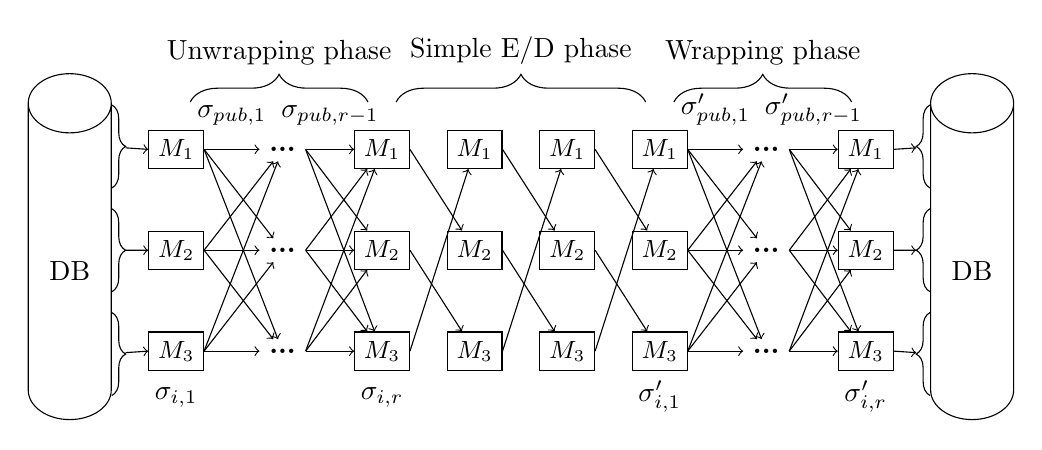
\begin{tikzpicture}[auto,
thin, 
scale=0.5,
block/.style={draw, fill=white, rectangle, font=\small}]

\node[draw, cylinder, shape border rotate=90, anchor = west, minimum height=12.5em, minimum width=3em] 		(0)		{$\text{DB}$};

\node[block, align=center]							(B0)[right of=0, yshift=.75em,  xshift=1em ]		{$M_2$};
\node[block, anchor= north, align=center]			(A0)[above of=B0, yshift=0.8em ]	{$M_1$};
\node[block, anchor = south, align=center,label=below:{\color{white}'\color{black}$\sigma_{i,1}$\color{white}'}]			(C0)[below of=B0, yshift=-0.8em]	{$M_3$};

\node[draw=none, fill=none]    		(XB1)[right of=B0, xshift=1em]	{\textbf{...}};
\node[draw=none, fill=none]    		(XA1)[right of=A0, xshift=1em]	{\textbf{...}};
\node[draw=none, fill=none]    		(XC1)[right of=C0, xshift=1em]	{\textbf{...}};

\node[block, align=center]							(B3)[right of=XB1,  xshift=.75em ]		{$M_2$};
\node[block, anchor= north, align=center]			(A3)[above of=B3, yshift=0.8em ]	{$M_1$};
\node[block, anchor = south, align=center,label=below:{\color{white}'\color{black}$\sigma_{i,r}$\color{white}'}]			(C3)[below of=B3, yshift=-0.8em]	{$M_3$};

\node[block, align=center]							(B4)[right of=B3,  xshift=0.5em ]		{$M_2$};
\node[block, anchor= north, align=center]			(A4)[above of=B4, yshift=0.8em ]	{$M_1$};
\node[block, anchor = south, align=center]			(C4)[below of=B4, yshift=-0.8em]	{$M_3$};

\node[block, align=center]							(B5)[right of=B4,  xshift=0.5em ]		{$M_2$};
\node[block, anchor= north, align=center]			(A5)[above of=B5, yshift=0.8em ]	{$M_1$};
\node[block, anchor = south, align=center]			(C5)[below of=B5, yshift=-0.8em]	{$M_3$};

\node[block, align=center]							(B6)[right of=B5,  xshift=0.5em ]		{$M_2$};	
\node[block, anchor= north, align=center]			(A6)[above of=B6, yshift=0.8em ]	{$M_1$};
\node[block, anchor = south, align=center,label=below:{$\sigma_{i,1}'$}]			(C6)[below of=B6, yshift=-0.8em]	{$M_3$};

\node[draw=none, fill=none]    		(XB7)[right of=B6, xshift=1em]	{\textbf{...}};
\node[draw=none, fill=none]    		(XA7)[right of=A6, xshift=1em]	{\textbf{...}};
\node[draw=none, fill=none]    		(XC7)[right of=C6, xshift=1em]	{\textbf{...}};

\node[block, align=center]							(B9)[right of=XB7,  xshift=.75em ]		{$M_2$};
\node[block, anchor= north, align=center]			(A9)[above of=B9, yshift=0.8em ]	{$M_1$};
\node[block, anchor = south, align=center,label=below:{$\sigma_{i,r}'$}]			(C9)[below of=B9, yshift=-0.8em]	{$M_3$};

\node[draw, cylinder, shape border rotate=90, anchor = east, minimum height=12.5em, minimum width=3em] 	(00)[right of=B9, xshift=1em, yshift=-.75em]				{$\text{DB}$};

\draw[decoration={brace, amplitude=1em}, decorate]  ([yshift=2em,xshift=-1em]A0.north east) -- ([yshift=2em, xshift=1em]A3.north west) node[above, pos=0.5, yshift=1em] {Unwrapping phase};

\draw[decoration={brace, amplitude=1em}, decorate]  ([yshift=2em,xshift=-1em]A3.north east) -- ([yshift=2em,xshift=1em]A6.north west) node[above, pos=0.5, yshift=1em] {Simple E/D phase};

\draw[decoration={brace, amplitude=1em}, decorate]  ([yshift=2em,xshift=-1em]A6.north east) -- ([yshift=2em,xshift=1em]A9.north west) node[above, pos=0.5, yshift=1em] {Wrapping phase};

\draw[decoration={brace, amplitude=0.5em}, decorate]([yshift=12em]0.east) -- ([yshift=6em]0.east) node {};
\draw[decoration={brace, amplitude=0.5em}, decorate]([yshift=4.5em]0.east) -- ([yshift=-1.5em]0.east) node {};
\draw[decoration={brace, amplitude=0.5em}, decorate]([yshift=-3em]0.east) -- ([yshift=-9em]0.east) node {};

\draw[decoration={brace, mirror, amplitude=0.5em}, decorate]([yshift=12em]00.west) -- ([yshift=6em]00.west) node {};
\draw[decoration={brace, mirror, amplitude=0.5em}, decorate]([yshift=4.5em]00.west) -- ([yshift=-1.5em]00.west) node {};
\draw[decoration={brace, mirror, amplitude=0.5em}, decorate]([yshift=-3em]00.west) -- ([yshift=-9em]00.west) node {};


\path[->, midway]
 ([yshift=8.9em,xshift=1em]0.east) edge node				{} (A0.west)
 ([yshift=1.5em,xshift=1em]0.east) edge node						{} (B0.west)
 ([yshift=-5.9em,xshift=1em]0.east) edge node				{} (C0.west)

 (A0.east) edge node[above,yshift=0.5em]	{$\sigma_{pub,1}$} 	(XA1)
 (A0.east) edge node						{} 					(XB1)
 (A0.east) edge node						{} 					(XC1)
 (B0.east) edge node						{} 					(XA1)
 (B0.east) edge node						{} 					(XB1)
 (B0.east) edge node						{} 					(XC1)
 (C0.east) edge node						{} 					(XA1)
 (C0.east) edge node						{} 					(XB1)
 (C0.east) edge node						{} 					(XC1)
 
 (XA1.east) edge node[above,yshift=.5em]	{$\sigma_{pub,r-1}$} 	(A3)
 (XA1.east) edge node						{} 					(B3)
 (XA1.east) edge node						{} 					(C3)
 (XB1.east) edge node						{} 					(A3)
 (XB1.east) edge node						{} 					(B3)
 (XB1.east) edge node						{} 					(C3)
 (XC1.east) edge node						{} 					(A3)
 (XC1.east) edge node						{} 					(B3)
 (XC1.east) edge node						{} 					(C3)

 
 (A3.east) edge node						{}				 	(B4)
 (B3.east) edge node						{} 					(C4)
 (C3.east) edge node						{} 					(A4)
 (A4.east) edge node						{}				 	(B5)
 (B4.east) edge node						{} 					(C5)
 (C4.east) edge node						{} 					(A5)
 (A5.east) edge node						{}				 	(B6)
 (B5.east) edge node						{} 					(C6)
 (C5.east) edge node						{} 					(A6)
 
 (A6.east) edge node[above,yshift=.5em]	{$\sigma_{pub,1}'$}		(XA7)
 (A6.east) edge node						{} 					(XB7)
 (A6.east) edge node						{} 					(XC7)
 (B6.east) edge node						{} 					(XA7)
 (B6.east) edge node						{} 					(XB7)
 (B6.east) edge node						{} 					(XC7)
 (C6.east) edge node						{} 					(XA7)
 (C6.east) edge node						{} 					(XB7)
 (C6.east) edge node						{} 					(XC7)

 (XA7.east) edge node[above,yshift=.5em]	{$\sigma_{pub,r-1}'$}	(A9)
 (XA7.east) edge node						{} 					(B9)
 (XA7.east) edge node						{} 					(C9)
 (XB7.east) edge node						{} 					(A9)
 (XB7.east) edge node						{} 					(B9)
 (XB7.east) edge node						{} 					(C9)
 (XC7.east) edge node						{} 					(A9)
 (XC7.east) edge node						{} 					(B9)
 (XC7.east) edge node						{} 					(C9)
 
 (A9.east) edge node						{} 					([yshift=8.9em,xshift=-1em]00.west)
 (B9.east) edge node						{} 					([yshift=1.5em,xshift=-1em]00.west)
 (C9.east) edge node						{} 					([yshift=-5.9em,xshift=-1em]00.west);

\end{tikzpicture}
\end{minipage}
\centering
\caption{Parallel mix-net: Rebuild method (all phase) and Layered method (only the Wrapping phase) with 3 mixes.}\label{fig:Par}
\end{figure*}

\subsubsection{Parallel Layered scheme.}
In this design, chunks of the database are assigned to each mix which keep encrypting and permuting the records. Before the eviction, the database is permuted with the old seeds $\sigma_i$ and encrypted with the old encryption keys $k_i$. Afterwards, the records are encrypted with both $k_i$ and $k_i'$, permuted with both $\sigma_i$ and $\sigma_i'$, and the indices are saved in the record index. 
As no permutation layer is ever removed, the record indistinguishability assumption holds, the eviction can then consist of $r= m/2 \ \log(n/s)$ rounds. \\

\noindent\textit{Mix Instructions.}
The client need to send to each mix the session keys to access the database $(id,\ token)$, the total number of records $n$, the elements used to compute the encryption keys and permutation seeds $(\alpha_i, \beta_i)$, the number of rounds $r$, and the ordered $list=(ports,\ ips)$ of the mixes participating in the eviction. The client thus send :
$$C \rightarrow M_i\ :\ db,\ \alpha_i,\ \beta_{i},\ n,\ r,\ list$$

\noindent The encryption keys $k_i$ and the permutation seeds $\sigma$ are generated as follows :
\begin{align*}
\alpha_{i,0} &= g^{z_i}, &ss_{i,0 }&= y_{i,0}^{z_i}, &k_{i,0},\ \sigma_{i,0}&=hkdf(ss_{i,0})\\
\beta_{i, 0} &= g^{\Pi_{j\neq i}m_j}, &sk_0 &= \beta_{i,0}^{m_i}, &\sigma_{pub, 0}&=hkdf( sk_0)
\end{align*}

We furthermore refresh the permutation seeds and encryption keys at each round thanks to blinding the group elements. Let $h_b : \mathcal{G}^* \rightarrow \mathbb{Z}_{q}^*$ the hash function we use for computing blinding factors, we can then compute the $\alpha$ and $\beta$ for the round $j+1$ as follows:
\begin{align*}
b_{i,j+1}&=h_b(\alpha_{i,j}, ss_{i,j}), & \alpha_{i,j+1} &= g^{z_i\Pi_{k\leq j}b_{i,k}}\\
b_{pub,j+1}&=h_b(sk_{j}), &\beta_{i, j+1} &= g^{\Pi_{k\leq j}b_{pub,k}\Pi_{l\neq i}m_l}\\
\end{align*}

\noindent\textit{Mix operations.} In this scheme the mix $mix_i$ receive a list of encrypted record from all mixes (or the database). It first merges the record lists and  sorts them to the natural order thanks to the public seed. It then encrypts each record and permute them according to the private key and seed. It finally computes the record allocation arrays (c.f. Algorithm~\ref{alg:PRA}) before sending the records accordingly to them.\\

\noindent\textit{Client operations.} The client can find the record index locally as it was stored before the eviction. To decrypt a record, the client uses the same Layered Trial and Error algorithm, depicted in Algorithm~\ref{alg:ldec}, with the new number of rounds and a different function to retrieve the list of mixes storing the record during the different rounds.
The access method is the same as described in Algorithm~\ref{alg:lacc}. \\

\noindent\textit{Costs.} The mix communication cost is $ (r+2) \cdot n \cdot b$, the mix permutation cost is $m \log(n/s) \cdot C_{\Pi}(n/m)$ with $C_{\Pi}(n/m)$ the cost of permuting $n/m$ elements and the encryption cost $m/2 \log(n)\cdot  C_{cbc}$ with $C_{cbc}$ the cost of encrypting one data block. The client Lookup cost is of the order $O(1)$ as the indices, i.e. $n\log n$ bit, are stored locally. The client decryption cost will be talked in the evaluation (Section~\ref{Evaluation}), and the group elements stored on the client represents $2\kappa m$ bits.

\subsubsection{Parallel Rebuild method.}
When performing an eviction, the client assigns to each mix  $k=\frac{n}{m}$ distinct indexes together with a list of shared secrets from which will be derive public and private permutation seeds and encryption keys.

At first, the mixes fetch their allocated records from the database. They then unwrap the previous permutation: the last wrapping permutations are undone in reverse order thanks to the old private seeds and the records are decrypted with the old encryption keys before being distributed to all mixes according to the inverse permutation of the old public seeds. Then starts the wrapping, where the records are permuted according to the new seeds, encrypted with the new encryption keys and distributed to the mixes according to the new public seeds. Between the wrapping and unwrapping phases, the mixes exchanged in a cascade fashion their records and encrypt them with both the new and the old key.\\

\noindent\textit{Mix Instructions.}
The client sends the same instructions as in the Parallel Layered design but with double the amount of group elements $\alpha$, the old and the new ones. The message format is then : 
$$C \rightarrow M_i\ :\ db,\  \alpha_i,\ \alpha_i',\ \beta,\ \beta',\ n,\ r,\ list$$

To derive the permutation seeds $\sigma$ and encryption keys $k$, we make use of the random private elements $z,i$ and $m_i$, the public and private keys $y$ and $x$ as in the Layered method. We furthermore derive the $\alpha$ $r$ more times for the simple the Encryption/Decryption phase. 
\begin{align*}
b_{i,j+1}&=h_b(\alpha_{i,j}, ss_{i,j}), & \alpha_{i,j+1} &= g^{z_i\Pi_{k\leq j}b_{i,k}}\\
b_{pub,j+1}&=h_b(y_c, sk_{j}), &\beta_{i, j+1} &= g^{\Pi_{k\leq j}b_{pub,k}\Pi_{l\neq i}m_l}\\
\end{align*}

\noindent\textit{Mix Operations.} During the first $r$ rounds, the records are first sorted, then  unwrapped (permuted and decrypted with the old keys and seeds) and sent to the mix-net according to the public record allocation. Then the groups of $n/m$ records are encrypted and decrypted in $m$ parallel cascades. Finally, the records are sorted, wrapped (encrypted and permuted with the new ones) and sent to the mix-net according to the public allocation during the last $r$ rounds.\\

\noindent\textit{Client Operations.} To access and decrypt a record, the client uses the same algorithms as in the Cascade Rebuild scheme but decrypt for $m$ more rounds.  To recover a record remote position, the client derive from the $m+1$ group elements the permutation seeds used during the $r$ rounds of operations as depicted in Algorithm~\ref{alg:PIL} with the last index in the indices array being the one sought.

\noindent\textit{Costs.} The mix communication cost is $ (2m+r+2) \cdot n \cdot b$, the mix permutation cost is $8m \log n \cdot C_{\Pi}(n/m)$ with $C_{\Pi}(n/m)$ the cost of permuting $n/m$ elements and the encryption cost $n (4 \log n +2) \cdot C_{ctr}$ with $C_{ctr}$ the cost of encrypting one data block. The client Lookup cost is of the order $m (C_{\Pi}(n)+C_{\Pi}(n/m))$. The client decryption cost is $(r+m) C_{ctr}$, and the group elements stored on the client represents $2\kappa (m+1)$ bits.

\section{Security Argument}\label{Security}

We first remark that all of the eviction meta data is independent of data content, as it is entirely determined by the sole parameter $n$. The mix instructions are never shared between mixes and never shared with the database, the encryption keys and permutation seeds thus remain secret and are refreshed at every round. The data content is also never revealed to the adversary and is refreshed upon reception by every mix.

\noindent\textbf{Cascade mix-net.}
In this architecture, the whole database passes by every mix including the honest one where it is locally permuted and re-encrypted with the private shared keys. As a polynomial adversary cannot break the PRF, the database order is kept confidential.\\

\noindent\textbf{Parallel mix-net.}
In this design, chunks of the database are exchanged between mixes during $r=2m\log(n)$ rounds. The adversary can benefit of the fact that some records may never go to the honest mixes (with probability $p=(e^{-r/m} << 1$).\\

For the \emph{Rebuild method}, we derived use Goodrich in 2012~\cite{goodrich2012anonymous} to quantify the information leakage (see Appendix~\ref{proof:pmn}) and found that the number of rounds the mix-net is asked to shuffle the records is sufficient to bound the expected sum of square error between the card assignment probabilities and the uniform distribution by at most $1/n^b$.

For the \emph{Layered method}, we proposed to use the previous randomness to reduce the number of rounds needed to be close to the uniform distribution. We can also reuse Goodrich's proof by changing the probabilities such that $w_i(t)$ being now the probability the $i^{th}$ record at the $t^{th}$ round was in the cache at first and $\Phi(t)=\Sigma w_i(t) - s/n$, we obtain $r>m\log(n/s)$.


\section{Evaluation}\label{Evaluation}
\textbf{Layered method.} We look here at the average number of encryption layers $e$ a record has before being decrypted. Making the assumption that the record access distribution is uniform, we can represent the problem of accessing all records at least once as a coupon collector problem. In that case, we expect $E[e_{all}]\leq(n/s)\cdot H_n$ evictions before all records have been fetched once with $H_n$ the $n^{th}$ harmonic number. The expected number of encryption layers per record before decryption is however $E[e]\leq{r/s} \cdot \left ( \frac{n+1}{2}\cdot(H_n-1/2)+1/2 \right )$. For $n=10^6$ and $s=\sqrt{n}$, we have $E[e]\approx 15 \cdot 10^3$ and $E[r]\approx 7\cdot 10^3 \cdot r$.
\begin{proof}
Lets $\tau_n$ be the random number of coupons collected when the first set contains every $n$ types. We have, $E[\tau_n]=n\sum_{i=1}^n \frac{1}{i} = n \cdot H_n$.
Since we fetch $s$ unique records per eviction (we cannot fetch a record already in the stash), the previous result is an upper bound of the number of requests needed and so the expected number of eviction is $E[e_{all}]\leq n/s\ H_n$.

We now want to find the average number of encryption layers per record before decryption, this is equivalent to finding the average number of evictions before a record is deciphered. 
Hence we have, $E[e]\leq r/s \cdot \sum_{i=1}^n E[\tau_i] = r/s\ \sum_{i=1}^n \left (\frac{(n+1-i)(n+i)}{2}\cdot \frac{1}{i}\right )$ from which can be calculated the result presented earlier. 
\end{proof}

To reduce these numbers, we modify the access method written in Algorithm~\ref{alg:lacc}. When the client requests a record from the database, $d$ other records are chosen uniformly at random from the set of unaccessed records. These records are then fetched, their encryption is refreshed as written previously and the client overwrites with these records their older version on the database. Doing so, with $d$ high enough, yields a better approximation of the uniform distribution assumption and we would obtain  $E[e_{all}]\leq n/(sd) \cdot H_n $ and $E[e] \leq {r/(sd)} \cdot \left [ \frac{n+1}{2}\cdot(H_n-1/2)+1/2 \right ] \ H_n$.
With $d=\sqrt n$, we now have $E[e_{all}]\leq 15 r$ and $E[e]\leq 7r$.

\begin{table*}
\centering
\begin{tabular}{l *4c}
\toprule
    					& Cascade - Layered	 			& Cascade - Rebuild							& Parallel - Layered 						& Parallel - Rebuild\\
\midrule
\#Rounds ($r$) & $m$ & $3m$ & $\frac{m}{2} \log\left( \frac{n}{s}\right)$ &  $4m\log(n) +  m$ \\
Mix Encryption cost & $m \cdot  n$ & $4m  \cdot  n$ & $\frac{n}{2} \log\left (\frac{n}{s}\right)$ & $n(4\log(n) + 2) $ \\
Mix Permutation cost & $m n \cdot C_{\Pi}(n)$ & $2 m n C_{\Pi}(n)$ & $m \log\left (\frac{n}{s}\right)\cdot C_{\Pi}\left(\frac{n}{m}\right)$ & $8m\log(n) \cdot C_{\Pi}\left ( \frac{n}{m} \right )$ \\
Mix Communication cost & $(m+1) \cdot C_{com}(n)$ & $r \cdot C_{com}(n)$ & $m(r+2) \cdot C_{com}\left(\frac{n}{m}\right)$ & $m(2r+m+2) \cdot C_{com}\left(\frac{n}{m}\right)$\\
Client Lookup cost & $O(1)$ & $m\cdot C_{\Pi}(n)$ & $O(1)$ & $m \cdot [C_{\Pi}\left ( \frac{n}{m}\right )h+ 2C_{\Pi}(n)]$\\
Client Decryption cost & $\sim \frac{nr}{2s} H_n$ & $2m$ & $\sim \frac{nr}{2s} H_n$ & $2m$\\
Client Additional storage & $n\log(n)+ 2 \kappa m$ & $km$ &$n\log(n)+ 2 \kappa  (m+1)$ & $2 \kappa  (m+1)$ \\
\bottomrule
\end{tabular}
\centering
\caption{Cost comparison of the designs with $C_{E}$ the cost of 1 encryption, $C_{\Pi}(x)$ the permutation cost and $C_{com}(x)$ the communication cost of $x$ records in the scheme.}
\end{table*}

\subsection{Comparison}\label{Comparison}
Comparison of our schemes.
We did not include the record allocation cost in the tables as it can be done while waiting for the records.

For the cascade architecture, all the costs are linear in the number of mixes.
For the parallel architecture, no computation cost depends on $m$ (considering that $C_E \gg C_{\Pi}$), we could "nearly" say it for the communication cost \george{}
The parallel architecture can be faster than the cascade one. For most database depending on the the underlying ORAM system (on $s$) (if $m \geq 1/2 \log(\frac{n}{s})$), for the Layered method for small to medium sized databases for the Rebuild method (if $m \geq log(n) +1/2$).
The Layered method needs more additional space and decryption takes longer than for the Rebuild method, however the eviction is faster \raphael{at least if the cost induced by the additional bytes for the Layered method is insignificant}.

\subsection{Implementation, Benchmark and Performances}\label{Implementation}

\raphael{Ania example} We implement the system prototypes in ?? lines of Python 2.7 code for mix nodes, providers and clients, including unit-tests, deployment, and orchestration code, the source code being available under an open-source license5. We use the Twisted 15.5.0 network library for networking and the cryptographic tools from the petlib7 library. Thus, we implement Loopix as a multi-thread system, with cryptographic processing happening in a thread pool separated from the rest of the operations in the main thread loop. 

Experimental Setup. We present an experimental performance evaluation of the systems running on the AWS EC2 platform. All mix nodes run as separate instances on ??? instances running EC2 Linux on ?? machines with ?? RAM memory. 
 
\begin{table}[H]
\centering
\begin{tabular}{l *3c}
\toprule
    					& 3 mixes	  	& 5 mixes		& 7 mixes	\\
\midrule
Cascade Layered  	& 0 				& 0 				& 0 			\\
Cascade Rebuild  	& 0 				& 0 				& 0 			\\
Parallel Layered 	& 0 				& 0 				& 0 			\\
Parallel Rebuild  	& 0 				& 0 				& 0 			\\
\bottomrule
\end{tabular}
\centering
\caption{Performance (s) of the designs for the eviction of xxx records of yykbit.}
\end{table}

\iffalse
\section{Acknowledgement}
Danezis was supported by H2020  PANORAMIX Grant (ref. 653497) and EPSRC Grant EP/M013286/1; and Toledo by Microsoft Research.
\fi

\section{Conclusion}\label{Conclusion}
New ORAM with mix-net ; amortizable eviction ; can fetch while eviction running ; multi-user friendly as all the secrets are on the server



\pagebreak
\bibliographystyle{splncs03}
\bibliography{mix_oram}

\pagebreak
\section{Appendix}
\subsection{Proof $k$-RTS}\label{proof:kRTS}
\begin{proof}
To prove the upper bound, we use Diaconis et al. method ~\cite{aldous1986shuffling} which consists in marking cards depending on whether they have already been picked or not. Let's define $\tau$ the stopping time, i.e. the time when every card has been marked and $\tau_i$ the number of transpositions before $i$ cards have been marked. The $\tau_i$ are independent geometric variables with probability of success $p_t$ as implied by the game rules.
We thus have,
\begin{align*}
 p_t &= \sum_{i=1}^{min(k,n-t)} {k \choose i} \cdot {t+1 \choose i} \cdot {n-t \choose i}\cdot{n \choose i}^{-2}&\\
 &= \frac{1}{n^2} \cdot \left ( k \cdot (t+1)\cdot(n-t) + \alpha_{n,t,k}\right ),\ \text{with positive } \alpha_{n,t,k} = \mathcal{O}\left(n^{-k}\right )
\end{align*}

We can thus rewrite $\tau$'s expectation as following.
\begin{align*}
 E(\tau) &=  E \left ( \sum_{i=0}^{n-1} \tau_i \right ) = \sum_{t=0}^{n-1} \frac{1}{p_{t}}  < \sum_{t=0}^{n-1} \frac{n^2}{k \cdot (t+1)\cdot(n-t)}&\\  
 &< \frac{2}{k} \cdot \frac{n^2}{n+1} \cdot \left( \ln(n) + \gamma +\mathcal{O}(\frac{1}{n}) \right),\ \gamma = \lim_{n \to \infty} H_n - \ln(n)& \\
 \end{align*}
 \end{proof}
 \vspace{-2.5em}
 
\subsection{Proof of Oblivious Merge}\label{proof:OM}
\begin{proof}
We want to find the mixing time $\tau(\epsilon)$ of our oblivious merge of two sets of indistinguishable elements. To do so, we use the bound of the mixing time of an irreducible ergodic Markov Chain, where $p = \frac{1}{|V|}$, with the volume $V={n \choose s}$, and $1-\lambda^*$ is the spectral gap, we thus have,
$$\frac{\lambda^*}{1-\lambda^*} \cdot \log\left(\frac{1}{2 \epsilon} \right)\leq \tau(\epsilon) \leq \frac{1}{1-\lambda^*}\cdot \log \left( \frac{1}{2 \epsilon \cdot \sqrt{p}}\right) $$

We now represent the arranging of merge of the 2 distinct sets by the graph $\mathcal{G}$, a $k$-regular graph with $v$ vertices corresponding to the different orderings and the undirected edges to transpositions of two elements.
By definition, the eigenvalues of the transition matrix of the $\mathcal{G}$ are $k={\lambda'}_0 > {\lambda'}_1 \geq  ... \geq {\lambda'}_{n-1}$, and we have,
$$\text{diam}\left( \mathcal{G}\right) \leq \frac{log(v-1)}{log(\frac{k}{{\lambda'}^*})}+1 \text{ with } {\lambda'}^* = max_{i\neq0}({\lambda'}_i)= k \cdot \lambda^*$$
From which we can deduce that $ {\lambda}^* \geq \left ({n \choose s}-1 \right )^{\frac{1}{1-s}} \geq \left (\frac{n\cdot e}{s} \right )^{\frac{s}{1-s}} $ since $diam\left( \mathcal{G} \right)=s$ the diameter of the graph, $v= {n \choose s}$ the number of vertices and $k=s\cdot(n-s)$.

To find an upper-bound of $\lambda^*$, we will now look at spectral gap bounding.
Let's $\mathcal{G}_{0,1}=\{0,1\}^n$ be the group of elements with the XOR operation and $\mathcal{S}=\{x \in \mathcal{G},\ weight(x)=s\}$ the symmetric subset of $\mathcal{G}$ of n-binary array with $s$ 1s and $n-s$ 0s.
We call $Cay_{n,s}=Graph\left(  \mathcal{G}_{0,1}, \mathcal{S} \right) $ the Cayley graph generated from these structures.

\begin{lemma}
Let $\mathcal{G}$ be a finite Abelian group, $\chi\ :\  \mathcal{G} \rightarrow \mathbb{C}$ be a character of $\mathcal{G}$, $\mathcal{S} \subseteq \mathcal{G}$ be a symmetric set.
Let $M$ be the normalized adjacency matrix of the Cayley graph $G = Cay(\mathcal{G},\mathcal{S})$.
Consider the vector $x \in \mathbb{C}^\mathcal{G}$ such that $x_a = \chi(a)$. Then x is an eigenvector of $G$, with eigenvalue $$ \frac{1}{\mathcal{S}} \sum_{s\in \mathcal{S}} \chi\left(s\right)$$
\end{lemma}

\begin{theorem}
The Cayley graph $Cay_{n,s}$ has for eigenvalues $\mu_0 = 1 > \mu_1 \geq ... \geq \mu_{n-1}$ with, 
$$\mu_r = \frac{1}{\left | \mathcal{S} \right |} \sum_{i=1}^{min(r, n-r)} \left ( -1 \right )^i {r \choose i}{n-r \choose s-i}\\$$
\end{theorem}

\begin{subproof}
$\forall r \in \{0,1\}^n$, with $\chi_r(x)=\left ( -1 \right )^{\sum r_i \cdot x_i}$, we have,
\begin{align*}
\mu_r &= \frac{1}{\mathcal{S}} \sum_{s\in \mathcal{S}} \chi\left(s\right) = \frac{1}{\left | \mathcal{S} \right |} \sum_{s\in \mathcal{S}} \left ( -1 \right )^{\sum r_i \cdot s_i} = \frac{1}{\left | \mathcal{S} \right |} \sum_{i=1}^{min(r, s)} \left ( -1 \right )^i {r \choose i}{n-r \choose s-i} \\
\end{align*}
\end{subproof}

Remark. We recognize here the Vandermonde identity with alternating numbers. We argue that the eigenvalues of the Cayley graph $Cay_{n,s}$ are all positive as the smallest eigenvalue is null.
For $r=n-r$, the expression simplifies to $\mu_r = {r \choose \frac{n}{2}}$ if $n$ even, 0 otherwise.
For $r=1$, the expression simplifies to $\mu_1 = 1 - 2\cdot \frac{s}{n}$, the spectral gap of $Cay_{n,s}$ is thus equal to $2\cdot \frac{s}{n}$.\\\

We notice that the first graph $\mathcal{G}$ actually is a sub-graph of $Cay_{n,s}$ and as such the adjacent matrix of the first graph is included in the second's.
For $s>1$, $Cay_{n,s}$ is divided in two sub-graphs representing the cosets of $\{0,1\}^n$ as $\mathcal{S}$ is not a generating group of $\mathcal{G}_{0,1}$, $\mathcal{G}$ is only contained in one of the sub-graphs.
We use the Cauchy's Interlace Theorem to bound the eigenvalues of $\mathcal{G}$ with the ones of $Cay_{n,s}$,.

\begin{theorem}
Let $M$ be a Hermitian $n \times n$ matrix with eigenvalues ${\mu'}_0\geq ... \geq {\mu'}_{n-1}$ and $N$ a $m \times m$ sub-matrix of $M$ with eigenvalues ${\lambda'}_0\geq ... \geq {\lambda'}_{m-1}$ , we have
$$ {\mu'}_i \geq {\lambda'}_i \geq {\mu'}_{n-m+i+1} $$
\end{theorem}

We are here only interested in an upper-bound of $\lambda*$, as we have $\mu_{2^n+2-{n \choose s}}\leq \lambda_1\leq 1-2\frac{s}{n}$ and $0 \leq \lambda_n \leq \mu_2$, $\lambda* \leq 1-2\frac{s}{n}$. We thus have $\frac{1}{1-\lambda*}\leq\frac{n}{2\cdot s}$ and $\log {n \choose s} \approx s(\log(n/s-0.5)+1) -1/2\log(2\pi s)$ when $n \gg s$.
\end{proof}

\subsection{Proof of Parallel mix-net}\label{proof:pmn}
\begin{proof}
This proof is derived from Goodrich et al~\cite{goodrich2012privacy} who bounded the closeness of a shuffle to the uniform distribution using a compromised parallel mix-net. 

Let $w_i(t)$ the probability the $i^{th}$ record at the $t^{th}$ round was the first record at start, the sum of square metric $\Phi(t)=\Sigma_{i=1}^n (w_i(t)-1/n)^2$, $n$ the number of cards, $m$ the number of mixes out of which $m_a$ are corrupted and $k=n/m$.

We have by recurrence that the potential $\Delta\Phi^*$ changes when a group of K card is shuffled during a round as following : $\Delta\Phi^*=\Sigma_{1\leq i\leq n}(w_i-w_j)^2$.
Thereby,

\vspace{-1em}

\begin{align*}
E[\Delta\Phi] & = \frac{m}{n} \sum_{1\leq i\leq n} \Pr((i,j)\ in\ the\ same\ honest\ mix) (w_i-w_j)^2\\
&=\frac{k-1}{k(n-1)}\cdot \frac{m-m_a}{m} \sum_{i<j}(w_i-w_j)^2 \\\
E[\frac{\Delta\Phi}{\Phi}]&=\frac{(m-m_a)(k-1)}{2n(n-1)}\frac{\sum_{i,j}((w_i-1/n)-(w_j-1/n))^2}{\sum_k (w_k-1/n)^2}\\
&=\frac{(m-m_a)(k-1)}{n-1} \text{ since $\sum_k w_k -1/n=0$}
\end{align*}

We thus find,
\vspace{-1em}
\begin{align*}
E[\Phi(t+1)] &= (1-\frac{(m-m_a)(k-1)}{n-1}) E[\Phi(t)]\\
E[\Phi(t)]&= (1-\frac{(m-m_a)(k-1)}{n-1})^t
\end{align*} 

We want to find the conditions on $c$ such that the corrupted parallel mix-net can mix in $t=bc\log(n)$  such that $E[\Phi(t)]< n^{-b}$.
\vspace{-.75em}
\begin{align*}
E[\Phi(t)] = (1-\frac{(m-m_a)(k-1)}{n-1})^t &< n^{-b}\\
c \cdot\log(1+ \frac{1}{\frac{n-1}{(m-m_a)(k-1)}- 1}) &> 1\\
\end{align*}
\vspace{-1em}
Using Taylor series, assuming that $n-1\gg(m-m_a)(k-1)$,  we finally get
\begin{align*}
&c \cdot (\frac{1}{\frac{n-1}{(m-m_a)(k-1)}- 1} +o(n/k)) > 1 \\
&c > \frac{n-1}{(m-m_a)(k-1)}- 1 \simeq \frac{m}{m-m_a} -o(1)\\
\end{align*}
Thus, when shuffling $n$ cards with n a parallel mix-net composed of $m$ mixes out of which $m_a$ were compromised, we need $t>b\cdot \frac{m}{m-m_a} \log(n) $ rounds before the expected sum of squares error $E[\Phi(t)]$ between the card assignment probabilities and the uniform distribution is at most $1/n^b$ for any fixed $b>1$.
\end{proof}

\end{document}